\documentclass{article}
\usepackage[T1,T2A]{fontenc}
\usepackage[utf8]{inputenc}
\usepackage[english,russian]{babel}

\usepackage[left=3cm,right=3cm,
    top=3cm,bottom=3cm,bindingoffset=0cm]{geometry}

\usepackage{graphicx}
\usepackage{color}
\usepackage{hyperref}
\usepackage{amsmath}

\usepackage{setspace}
\usepackage{indentfirst}
\usepackage{textcomp}
\usepackage{ifthen}
\usepackage{calc}

\title{Теория Вероятностей и Математическая Статистика\\
ФИИТ, 2 курс, 4 семестр}
\author{Лекция 4}

\begin{document}
\maketitle

\section{Случайное явление. Парадокс Бертрана}

Для того, чтобы иметь представление о случайном явлении, рассмотрим пример -- \textbf{парадокс Бертрана}:
\\


Имеется круг, в который вписан равносторонний треугольник. В круге наугад выбирается хорда. Нужно найти вероятность того, что эта хорда окажется больше стороны треугольника.

\begin{center}
    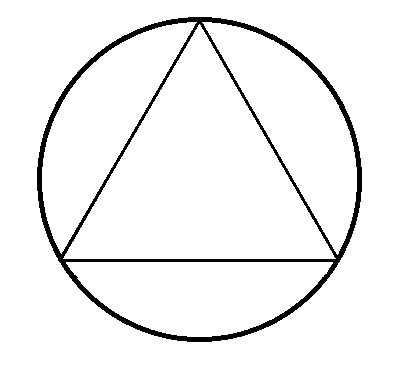
\includegraphics[scale=0.4]{1.png}
\end{center}

\begin{enumerate}
\item В первую очередь рассмотрим с выбором хорды наугад. Мы можем провести две различных хорды, и только на заштрихованной дуге у нас окажется хорда длиннее стороны треугольника. Соответственно, так как треугольник равносторонний, эта дуга занимает $\frac{1}{3}$, и итоговая вероятность $P = \frac{1}{3}$.

\begin{center}
    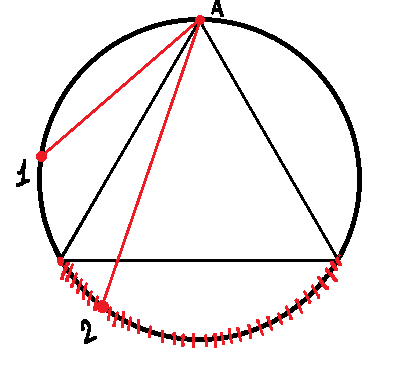
\includegraphics[scale=0.4]{2.png}
\end{center}

\item Построим дополнительный диаметр и несколько хорд. Соответственно, мы сможем выделить серединную область, где длина хорд будет больше длины стооны треугольника, а она займет половину круга, то есть вероятность $P = \frac{1}{2}$.

\begin{center}
    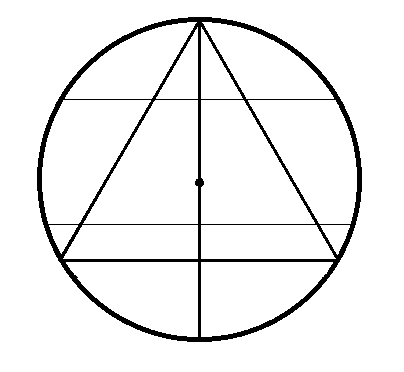
\includegraphics[scale=0.4]{3.png}
\end{center}

\item Рассмотрим еще один вариант! Выберем точку, которая будет центром хорды. Тогда, если мы будем ставить все подобные точки, то для нужных хорд мы сможем выделить область центров (закрашена на рисунке). Соответственно, отношение площадей круга даст нам нужную вероятность: $P = \frac{1}{4}$

\begin{center}
    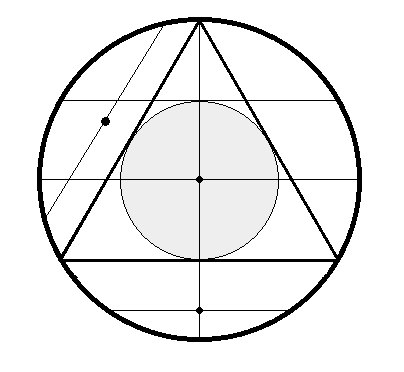
\includegraphics[scale=0.4]{4.png}
\end{center}

\end{enumerate}

\quad

Итого мы имеем целых 3 варианта. Интересно то, что все они правильные. Ключевым словом является \textbf{наугад}. И вариант выбора наугад, то есть сопоставление этому слову конкретной математической модели, определяет итоговое решение. В этом состоит и сложность этого парадокса.

\section{Случайные величины}

Эта тема -- вторая половина тем нашего семестра. Мы будем рассматривать, каким образам нашим случайным величинам можно сопоставить в соответствие некоторые числа.

Введем обозначения. Случайные величины будем обозначать греческими буквами: $\xi$ (кси); $\eta $ (эта), 

Большие латинские буквы $A, B, C$ -- события.

Прописная А -- $\mathcal{A}$ -- кл множеств ($\sigma$-алгебра).

$F, f, g$ -- функции.

$\tau, t, x, y, z$ -- переменные.

Мы будем работать в вероятностном пространстве $(\Omega, \mathcal{A}, P)$.
\\

\textbf{Определение.} Случайная величина $\xi$ заданная в вероятностном пространстве $(\Omega, \mathcal{A}, P)$ представляет собой функцию:

$$ \xi : \Omega \rightarrow \R ^1$$

Сопоставляет множество Так, что ${\omega : \xi(\omega) < x, x \in R ^ 1, y \in \mathcal(A)}$. 

Как и случайные события, случайная величина задается достаточно непросто. И для того, чтобы с этим дальше работать, нам потребуется еще одно распределение.

\textbf{Определение}. Функцией распределения случайной величины $\xi$: 

$$F_{\xi}(X) = F(x) = P({\omega : \xi(\omega) < x}) $$

Представляет собой вероятность ... для любых действительных $x$. Также можно записать и более кратко данное определение

$$ = P(\xi < x) $$

Поскольку $\xi$ является элементом $\sigma$-алгебры, значит вероятность существует всегда.

\subsection{Пример}

Три монеты. Мы знаем, что элементарные исходы будут следующие:

\begin{center}
0 0 0\\
0 0 1\\
0 1 0\\
0 1 1\\
1 0 0\\
1 0 1\\
1 1 0\\
1 1 1
\end{center}

Пусть $\xi$ -- кол-во гербов. Тогда различным исходам будет соответствовать различное колво гербов.

Постром функцию распределения $F(x)$. Рассмотрим конкретные точки:
\\

$F(-1) = P(\xi < -1)$ -- невозможно, так как множество значений у нас дискретное и конечное: $\{0, 1, 2, 3\} $.

$F(0) = P(\xi < 0)$ -- опять же, меньше нуля наша случайная величина быть не может.

$F(0.1) = P(\xi < 0.1) = P(\xi = 0) = \frac{1}{8}$

$F(0.7) = P(\xi < 0.7) = P(\xi = 0) = \frac{1}{8}$
\\

Из двух последних значений можно заметить, что нас интересуют точки изменения значений (дробей как выше мы можем подобрать сколько угодно для одного значения, на то у нас и функция).
\\

$F(1) = P(\xi < 1) = P(\xi = 0) = \frac{1}{8}$

$F(2) = P(\xi < 2) = P(\xi = 0) + P(\xi = 1) = \frac{4}{8}$

$F(3) = P(\xi < 3) = P(\xi = 0) + P(\xi = 1) + P(\xi = 2) = \frac{7}{8}$

$F(4) = P(\xi < 4) = P(\xi = 0) + P(\xi = 1) + P(\xi = 2) + P(\xi = 3) = 1$
\\

Таким образом, функция оказалась дискретной, кусочно-постоянной:

\begin{center}
    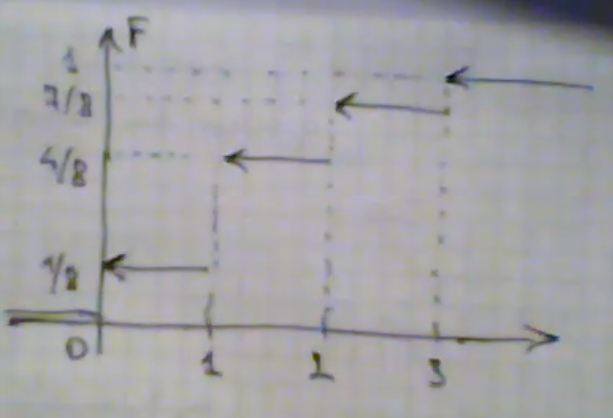
\includegraphics[scale=0.6]{5.png}
\end{center}

\subsection{Типы СВ}

Введем новые понятия:
\\

Случайная величина называется \textbf{дискретной случайной величиной} (ДСВ), если функция распределения СВ $F$ -- кусочно-постоянная.
\\

Случайная величина называется \textbf{абсолютно непрерывной (непрерывной) случайной величиной} (НСВ), если $F$ -- диффиренцируема почти во всех точках (за исключением конечного количества). 
\\

\textbf{Сингулярные случайные вличины} (ССВ) -- случайные величины, функции распределения которых не диффиренцируемы и к кусочно-постоянным функциям не относятся.

\begin{center}
    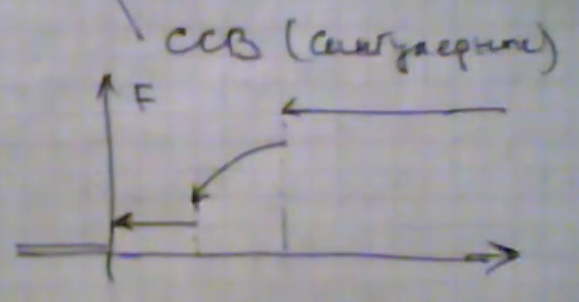
\includegraphics[scale=0.6]{6.png}
\end{center}


\subsection{ДСВ}

Величина $p_k = F(X_k + 0) - F(x_k)$ -- скачок функции распределения в точке разрыва.

Для предыдущего примера:

\begin{center}
    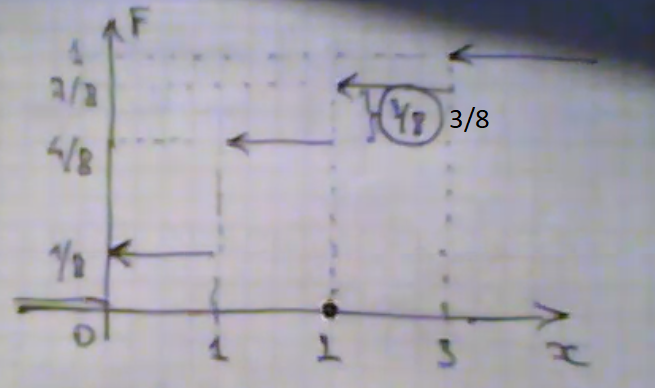
\includegraphics[scale=0.6]{7.png}
\end{center}

То есть вероятность $P(\xi = x_k) = p_k = F(X_k + 0) - F(x_k)$.
\\

Таким образом, дискретная случайная величина сосредоточенна в точках разрыва.

\subsection{НСВ}

Функция распределения допускает представления в виде:

$$ F(x) = \int\limits_{-\infty}^{x} f(t)dt$$

Тогда $f(x) = \frac{dF(x)}{dx}$, то есть производная. И называется она -- \textbf{плотность вероятности}.

\subsection{Свойства функции распределения случайной величины}

\begin{enumerate}
\item Ограниченность

$$0 \leq F(x) \leq 1$$

\item Неубывающая

$$x_1 < x_2 \Leftrightarrow F(x_1) \leq F(x_2)$$

\item Непрерывная слева

$$\lim\limits_{x \rightarrow x_0 - 0} F(x) = F(x_0)$$

\item Поведение на бесконечности

$$ \lim\limits_{x \rightarrow +\infty} F(x) = 1$$

$$ \lim\limits_{x \rightarrow -\infty} F(x) = 0$$

\end{enumerate}


\textbf{Замечание:} свойства 1-4 являются характеристическими. Любая функция, обладающая данными свойствами, является функцией рраспределения какой-либо случайной величины.

\subsubsection{Пример}

Найдем вероятность попадания случайной величины в полуинтервал:

$$P(\xi \in [a; b)) = P(a \leq \xi \leq b)$$

Для этого возьмем числовую прямую и представим ее в виде частей:

$$(-\infty; +\infty) = (-\infty; a)\cup[a; b)\cup[b; +\infty)$$

Из свойства 4 $\Rightarrow P(\xi \in (-\infty; +\infty)) = 1$

Значит, можем сделать следующее разложение:

$$= P(\xi \in (-\infty; a)) + P(\xi \in [a; b)) + P(\xi \in [b; +\infty)) = 1$$

Перепишем в виде неравенства:

$$ P(a \leq \xi \leq b) = 1 - P(\xi < a) - P(\xi \leq b)$$

Первое слогаемое -- значение распределение в точке $a$, то есть $F(a)$, а во втором слогаемом перейдем к событию противоположному:

$$ = 1 - F(a) - (1 - P(\xi < b)) = 1 - F(a) - 1 + F(b) = F(b) - F(a)$$

Таким образом, результат:

$$ P(a \leq \xi \leq b) = F(b) - F(a)$$
\\


Если выберем конкретную точку $c$: $P(\xi = c) = P(c \leq \xi < c + 0) = F(c + 0) - F(c)$:

\quadЕсли $F$ -- непрерывная функция, то $P(\xi = c) = 0$

\quadЕсли $F$ -- разрывна, а $c$ -- точка разрыва, то $P(\xi = c) \not= 0$ -- величина скачка в точке разрыва.
\\

Наша готовая формула очень похожа на формулу Ньютона-Лейбница. Так что:
если существует $f(x)$, то $p(A \leq (<) \xi \leq (<) b) = F(b) - F(a) = \int\limits_a^b f(x)dx$

\subsection{Плотность вероятности}

Таким образом плотность вероятности обладает следующими свойствами:

\begin{enumerate}
\item Неотрицательность

$$ f(x) \geq 0$$

\item Нормированность

$$ \int\limits_{-\infty}^{+\infty}f(x)dx = 1$$

\end{enumerate}

\subsection{Числовые характеристики случайной величины}

Так как работать с такими характеристическими функциями достаточно непросто, хочется исследовать возможность описание случайной величины через числовые характеристики. Конечно, полностью это не удастся, но в значительной степени это удастся.

\subsubsection{Математическое ожидание}

Одной из таких характеристик является -- \textbf{среднее значение} СВ (математическое ожидание):

$$M[\xi] = M\xi = \int\limits_{\Omega}\xi(\omega)P(d\omega)$$

Выражается через интеграл Лебега. Так как интеграл Римана не дает нам работать с разрывными функциями, мы будем пользоваться интегралом Лебега, в котором эти проблемы устранены. (Мы с его особенностями сталкиваться не будем, но все же определение полезно знать.)

В случае ДСВ или НСВ математическое ожидание можно вычислить пользуясь интегралом Стилтиеса (?):

$$M\xi = \int\limits_{\R}xdF(x)$$

\qquad$= \sum\limits_{k = 1}^{\infty}x_k p_k, p_k = F(x_k + 0) - F(x_k)$ -- ДСВ

\qquad$= \int\limits_{-\infty}^{+\infty}xf(x)dx$ -- НСВ
\\

Почему мат. ожидание не характеризует случайную величину полностью? Если рассматривать распределение точкек на отрезке $[-1, 1]$, то среднее значение, ожидаемо, $= 0$. Если мы рассмотрим ту же ситуацию на отрезке $[-100; 100]$ среднее значение тоже $0$, однако очевидно, что разброс значений намного больше.

Таким образом, мы хотим, чтобы лдна из числовых зарактеристик должна была бы говорить, насколько далеко отклоняются возможные случайные величины от ее среднего значения.

\subsubsection{Среднеквадратичное отклонение}

Средний квадрат отклонения от среднего значения случайной величины (дисперсия случайной величины).

Величину берем квадратичную, так как это позволит нам избавиться от знака.

$$M(\xi - M\xi)^2 = D[\xi] = D\xi$$

То, что внутри скобок -- отклонение случайной величины. После возведения в квадрат -- квадратичное отклонение случайной величины. А взятие среднего значения -- среднее квадратичное отклонение от среднего значения случайной величины. 

В случае ДСВ или НСВ дисперсия, это:

$$D\xi = \int\limits_{\R} (x - M\xi)^2dF(x) = $$

\qquad$= \sum\limits_{k = 1}^{\infty}(x_k - M\xi)^2 p_k$ -- ДСВ

\qquad$= \int\limits_{-\infty}{+\infty} = (x - M\xi)^2f(x)dx$ -- НСВ

\subsubsection{Свойства математического ожидания}

Математическое ожидание -- интеграл, а значит обладает всеми свойствами интеграла.

\begin{enumerate}

\item Математическое ожидание линейной неоднородной комбинации преобразовывется следующим образом:

$$M(a\xi + b) = a\cdotM\xi + b$$

\item Математическое ожидание для абсолютных величин связяно следующим неравенством

$$(M\xi) \leq M|\xi|$$
\end{enumerate}

\subsubsection{Свойства дисперсии}

\begin{enumerate}
\item Линейная комбинация

$$ D(a\xi + b) = M\Bigl[(a\xi + b) - M(a\xi + b)\Bigr]^2 = M\Bigl[a(\xi - M\xi)\Bigr]^2 = a^2 \cdot D\xi$$

\item Дисперсия -- величина неотрицательная

$$D\xi \geq 0 (D\xi = 0 \Leftrightarrow P(\xi = c) = 1)$$

\item Дисперсия -- это разность между средним значением квадрата и квадрата среднего значения (доказать можно самостоятельно)

$$ D\xi = M(\xi - M\xi)^2 = M\xi^2 - (M\xi)^2

\end{enumerate}

Также можно отметить, что размерность дисперсии -- квадратные единицы. А значит сравнивать со средним значением так просто не получится (а хотелось бы).

\textbf{Определение.} Среднее квадратическое отклонение $\sigma = \sqrt{D\xi}$ или $D\xi = \sigma^2 \geq 0$

\end{document}
